\section{Detecting buffer overflow}
Buffer overflow is historically one of the most common programming errors. It is the cause of security breaches, data corruption and program crashes. Detecting them is therefore preferred.\\\\
We start by defining a test case in the WHILE language, seen in figure \ref{code:array_example}.
\begin{figure}
  \begin{lstlisting}
program
[int A[2]]@$^1$@
[int i]@$^2$@
[i := -1]@$^3$@
while [i<3]@$^4$@ do
   [A[i] := i+1]@$^5$@
   [i := i+1]@$^6$@
od
end
 \end{lstlisting}
 \label{code:array_example}
 \caption{Code example for demonstrating buffer overflow}
\end{figure}

 \begin{figure}[h]
 \centering
 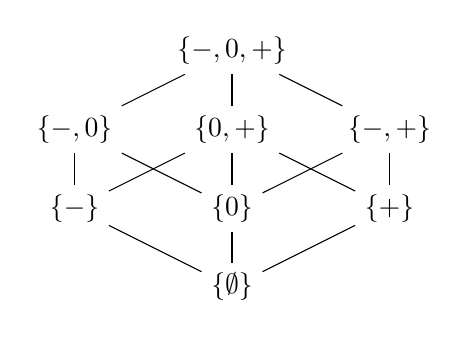
\begin{tikzpicture}
   \tikzstyle{line} = [draw, -latex'] 
   \node (nzp) at (2,3)  {$\{-,0,+\}$};
   \node (nz) at (0,2)  {$\{-,0\}$};
   \node (zp) at (2,2)  {$\{0,+\}$};
   \node (np) at (4,2)  {$\{-,+\}$};
   \node (n) at (0,1)  {$\{-\}$};
   \node (z) at (2,1)  {$\{0\}$};
   \node (p) at (4,1)  {$\{+\}$};
   \node (empty) at (2,0)  {$\{\emptyset\}$};
 
   \path [-] (nzp) edge (nz);
   \path [-] (nzp) edge  (np);
   \path [-] (nzp) edge  (zp);
 
   \path [-] (nz) edge (z);
   \path [-] (nz) edge (n);

   \path [-] (zp) edge (n);
   \path [-] (zp) edge (z);
   \path [-] (zp) edge (p);

   \path [-] (np) edge (z);
   \path [-] (np) edge (p);

   \path [-] (n) edge (empty);
   \path [-] (z) edge (empty);
   \path [-] (p) edge (empty);

 \end{tikzpicture}
  \caption{Complete lattice of sign detection instance}
 
  \label{fig:sign_detection_complete_lattice}
 \end{figure}

